%%=============================================================================
%% Methodologie
%%=============================================================================
\usepackage{multirow} % Add this in the preamble
\usepackage{longtable}
\usepackage[most]{tcolorbox}
\usepackage{array}
\usepackage{tikz}
\usepackage[margin=1in]{geometry}
\usepackage{pgfplots}
\usepackage{xcolor}


\chapter{\IfLanguageName{dutch}{Methodologie}{Methodology}}%
\label{ch:methodologie}

%% TODO: In dit hoofstuk geef je een korte toelichting over hoe je te werk bent
%% gegaan. Verdeel je onderzoek in grote fasen, en licht in elke fase toe wat
%% de doelstelling was, welke deliverables daar uit gekomen zijn, en welke
%% onderzoeksmethoden je daarbij toegepast hebt. Verantwoord waarom je
%% op deze manier te werk gegaan bent.
%% 
%% Voorbeelden van zulke fasen zijn: literatuurstudie, opstellen van een
%% requirements-analyse, opstellen long-list (bij vergelijkende studie),
%% selectie van geschikte tools (bij vergelijkende studie, "short-list"),
%% opzetten testopstelling/PoC, uitvoeren testen en verzamelen
%% van resultaten, analyse van resultaten, ...
%%
%% !!!!! LET OP !!!!!
%%
%% Het is uitdrukkelijk NIET de bedoeling dat je het grootste deel van de corpus
%% van je bachelorproef in dit hoofstuk verwerkt! Dit hoofdstuk is eerder een
%% kort overzicht van je plan van aanpak.
%%
%% Maak voor elke fase (behalve het literatuuronderzoek) een NIEUW HOOFDSTUK aan
%% en geef het een gepaste titel.

%\section{Oorzakenanalyse}
%Het onderzoek begint met een oorzakenanalyse, deze heeft als doel om het identificeren van de oorzaak/oorzaken van de lange A\&E wachttijden. Bij het uitvoeren van de oorzakenanalyse worden verschillende methodes toegepast om de kern van het probleem te identificeren, zoals een brainstormsessie in combinatie met de 5 Whys-methode \ref{fig:Figuur15}. Zodra diverse oorzaken geïdentificeerd zijn, begint er een analyse door middel van het Fishbone-model \ref{fig:Figuur15} om te voorkomen dat mogelijke onderliggende oorzaken over het hoofd worden gezien. Vervolgens wordt de oorzaak die het meest impact heeft op de wachttijden geïdentificeerd als de hoofdoorzaak. Tot slot zal er bepaald worden of IoT een oplossing kan zijn tot de hoofdoorzaak.  Verder in het onderzoek wordt er dieper bekeken naar welke IoT devices gebruikt kunnen worden in de gezondheidszorg, zodra de devices geselecteerd zijn, wordt er op een meer diepgaande wijze onderzocht of IoT een geschikte oplossing kan bieden.

%\begin{figure}[h]
%    \centering
%    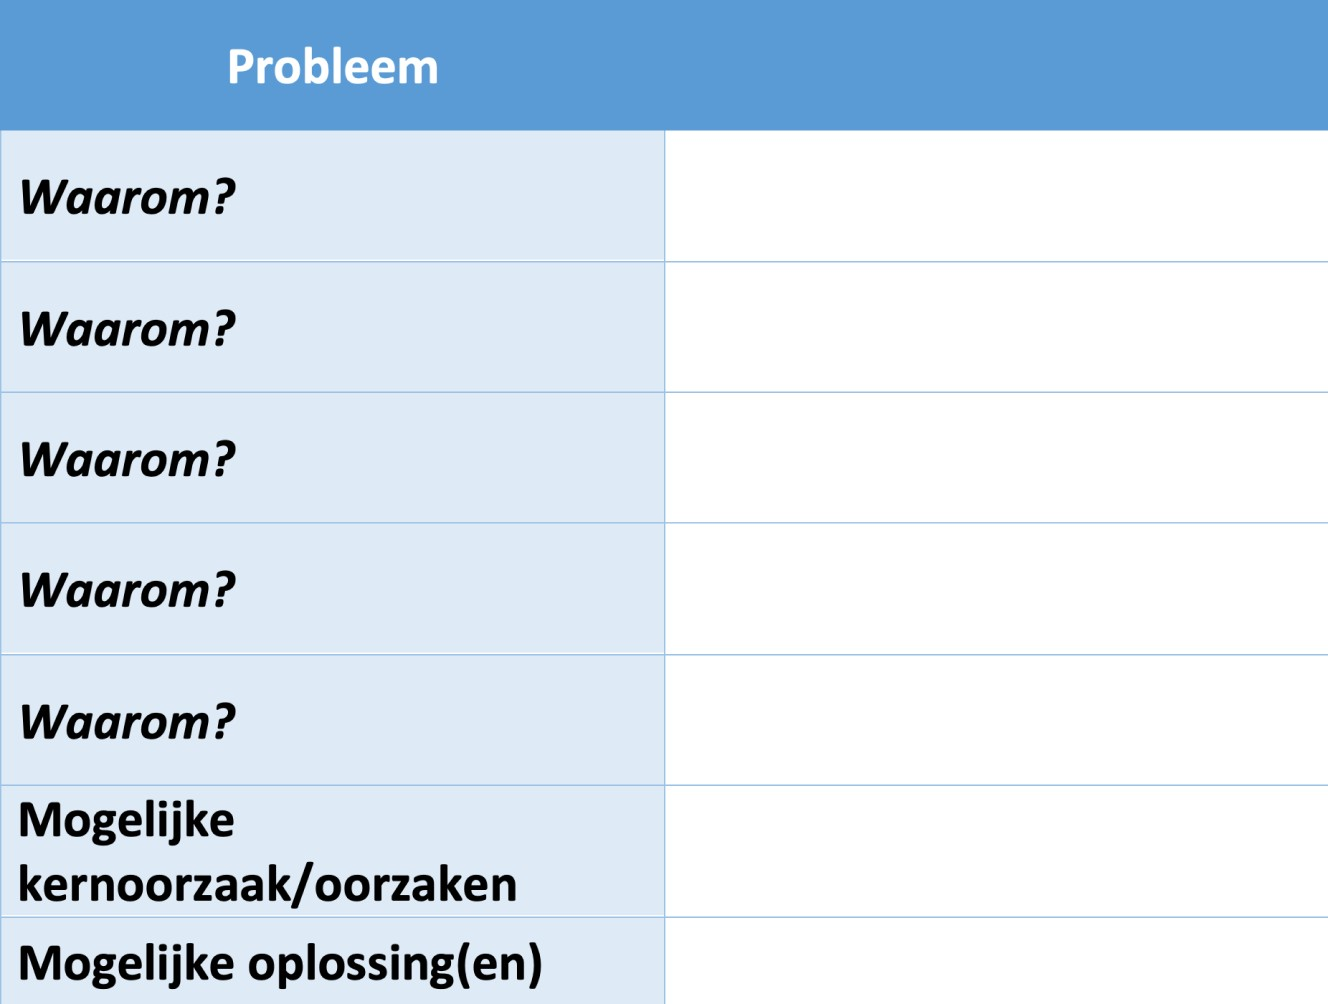
\includegraphics[width=0.5\textwidth]{img/Figuur-5}
%    \caption{5 Whys”-methode}
%    \label{fig:Figuur15}
%    \textit{Source: \autocite{Scharwaechter2023}}
%\end{figure}

%\begin{figure}[h]
%    \centering
%    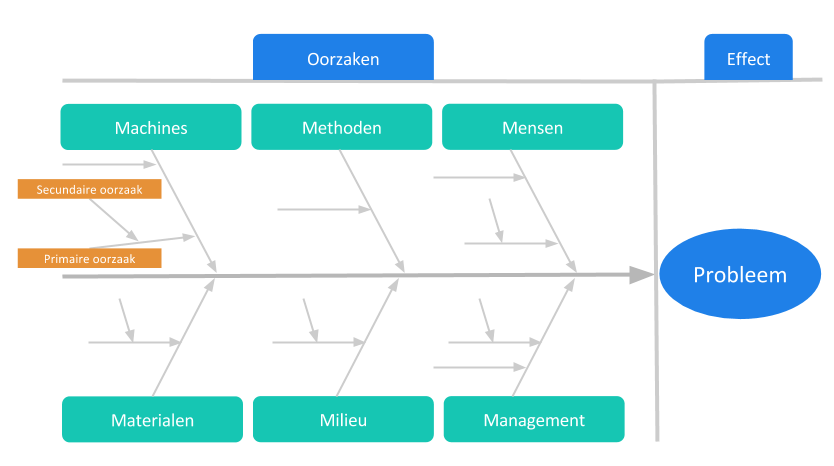
\includegraphics[width=0.7\textwidth]{img/Figuur-6}
%    \caption{De fishbone diagram}
%    \label{fig:Figuur16}
%    \textit{Source: \autocite{Swaen2023}}
%\end{figure}

%Doelstelling

%welke deliverables daar uit gekomen zijn

%welke onderzoeksmethoden je daarbij toegepast hebt

%Verantwoord waarom je op deze manier te werk gegaan bent

%Het onderzoek begint met het uitvoeren van een uitgebreide oorzakenanalyse. Dit is een fundamentele stap bij het identificeren van de oorzaak van de langdurige wachttijden binnen de A\&E afdelingen van ziekenhuizen. De analyse begint met het definiëren van het probleem. Om die reden wordt de “5 Whys”-methode toegepast samen met een brain\-storming-sessie. De “5 Whys”-methode wordt gebruikt om de kern van het probleem te achterhalen door telkens de vraag waar\-om te stellen, \ref{fig:Figuur5} en de oorzaak proberen te identificeren via de brain\-storming-sessie. Zodra diverse oorzaken geïdentificeerd zijn, begint er een analyse door middel van het Fishbone-model. De reden achter het gebruik van dit model is het voorkomen dat mogelijke onderliggende oorzaken over het hoofd worden gezien. Verder biedt het model simpliciteit bij het trekken van conclusies dankzij een visuele representatie tussen de categorisch weergegeven oorzaken en het probleem. Vervolgens is elke oorzaak zorgvuldig bestudeerd, degene die de grootste impact heeft op langdurige wachttijden is geselecteerd als de hoofdoorzaak. Een overweging is vervolgens gemaakt, om te achterhalen of IoT in het algemeen een oplossing kan zijn voor deze oorzaak. Verder in het onderzoek wordt er dieper bekeken naar welke IoT devices gebruikt kunnen worden in de gezondheidszorg, zodra de devices geselecteerd zijn, wordt er op een meer diepgaande wijze bekeken hoe de apparaten een oplossing kunnen zijn voor de hoofdoorzaak.

\section{Literatuurstudie over bestaande oplossingen}
Zie hoofdstuk \ref{ch:stand-van-zaken} voor een gedetailleerde literatuurstudie over bestaande IoT implementaties in de gezondheidszorg. \textit{Onder Internet of Things bij het verkorten van wachttijden in het gezondheidszorg}.

%\section{Geoptimaliseerde servicezones} %

%\begin{table}[h]
%    \centering
%    \tiny
%    \caption{Table with Type, Description, and Image}
%    \begin{tabular}{ | m{3cm} | m{6cm} | m{8cm} | }
%        \hline
%        \textbf{Type} & \textbf{Description} & \textbf{Image} \\ 
%        \hline
%        Type 1: Ziekenhuis/Spoed & Een wachtruimte van een bepaald ziekenhuis afdeling (cardiologie, ophtamologie, enz.. ) of een wachtruimte aan de bali/triage van een spoedafdeling.  & 
%        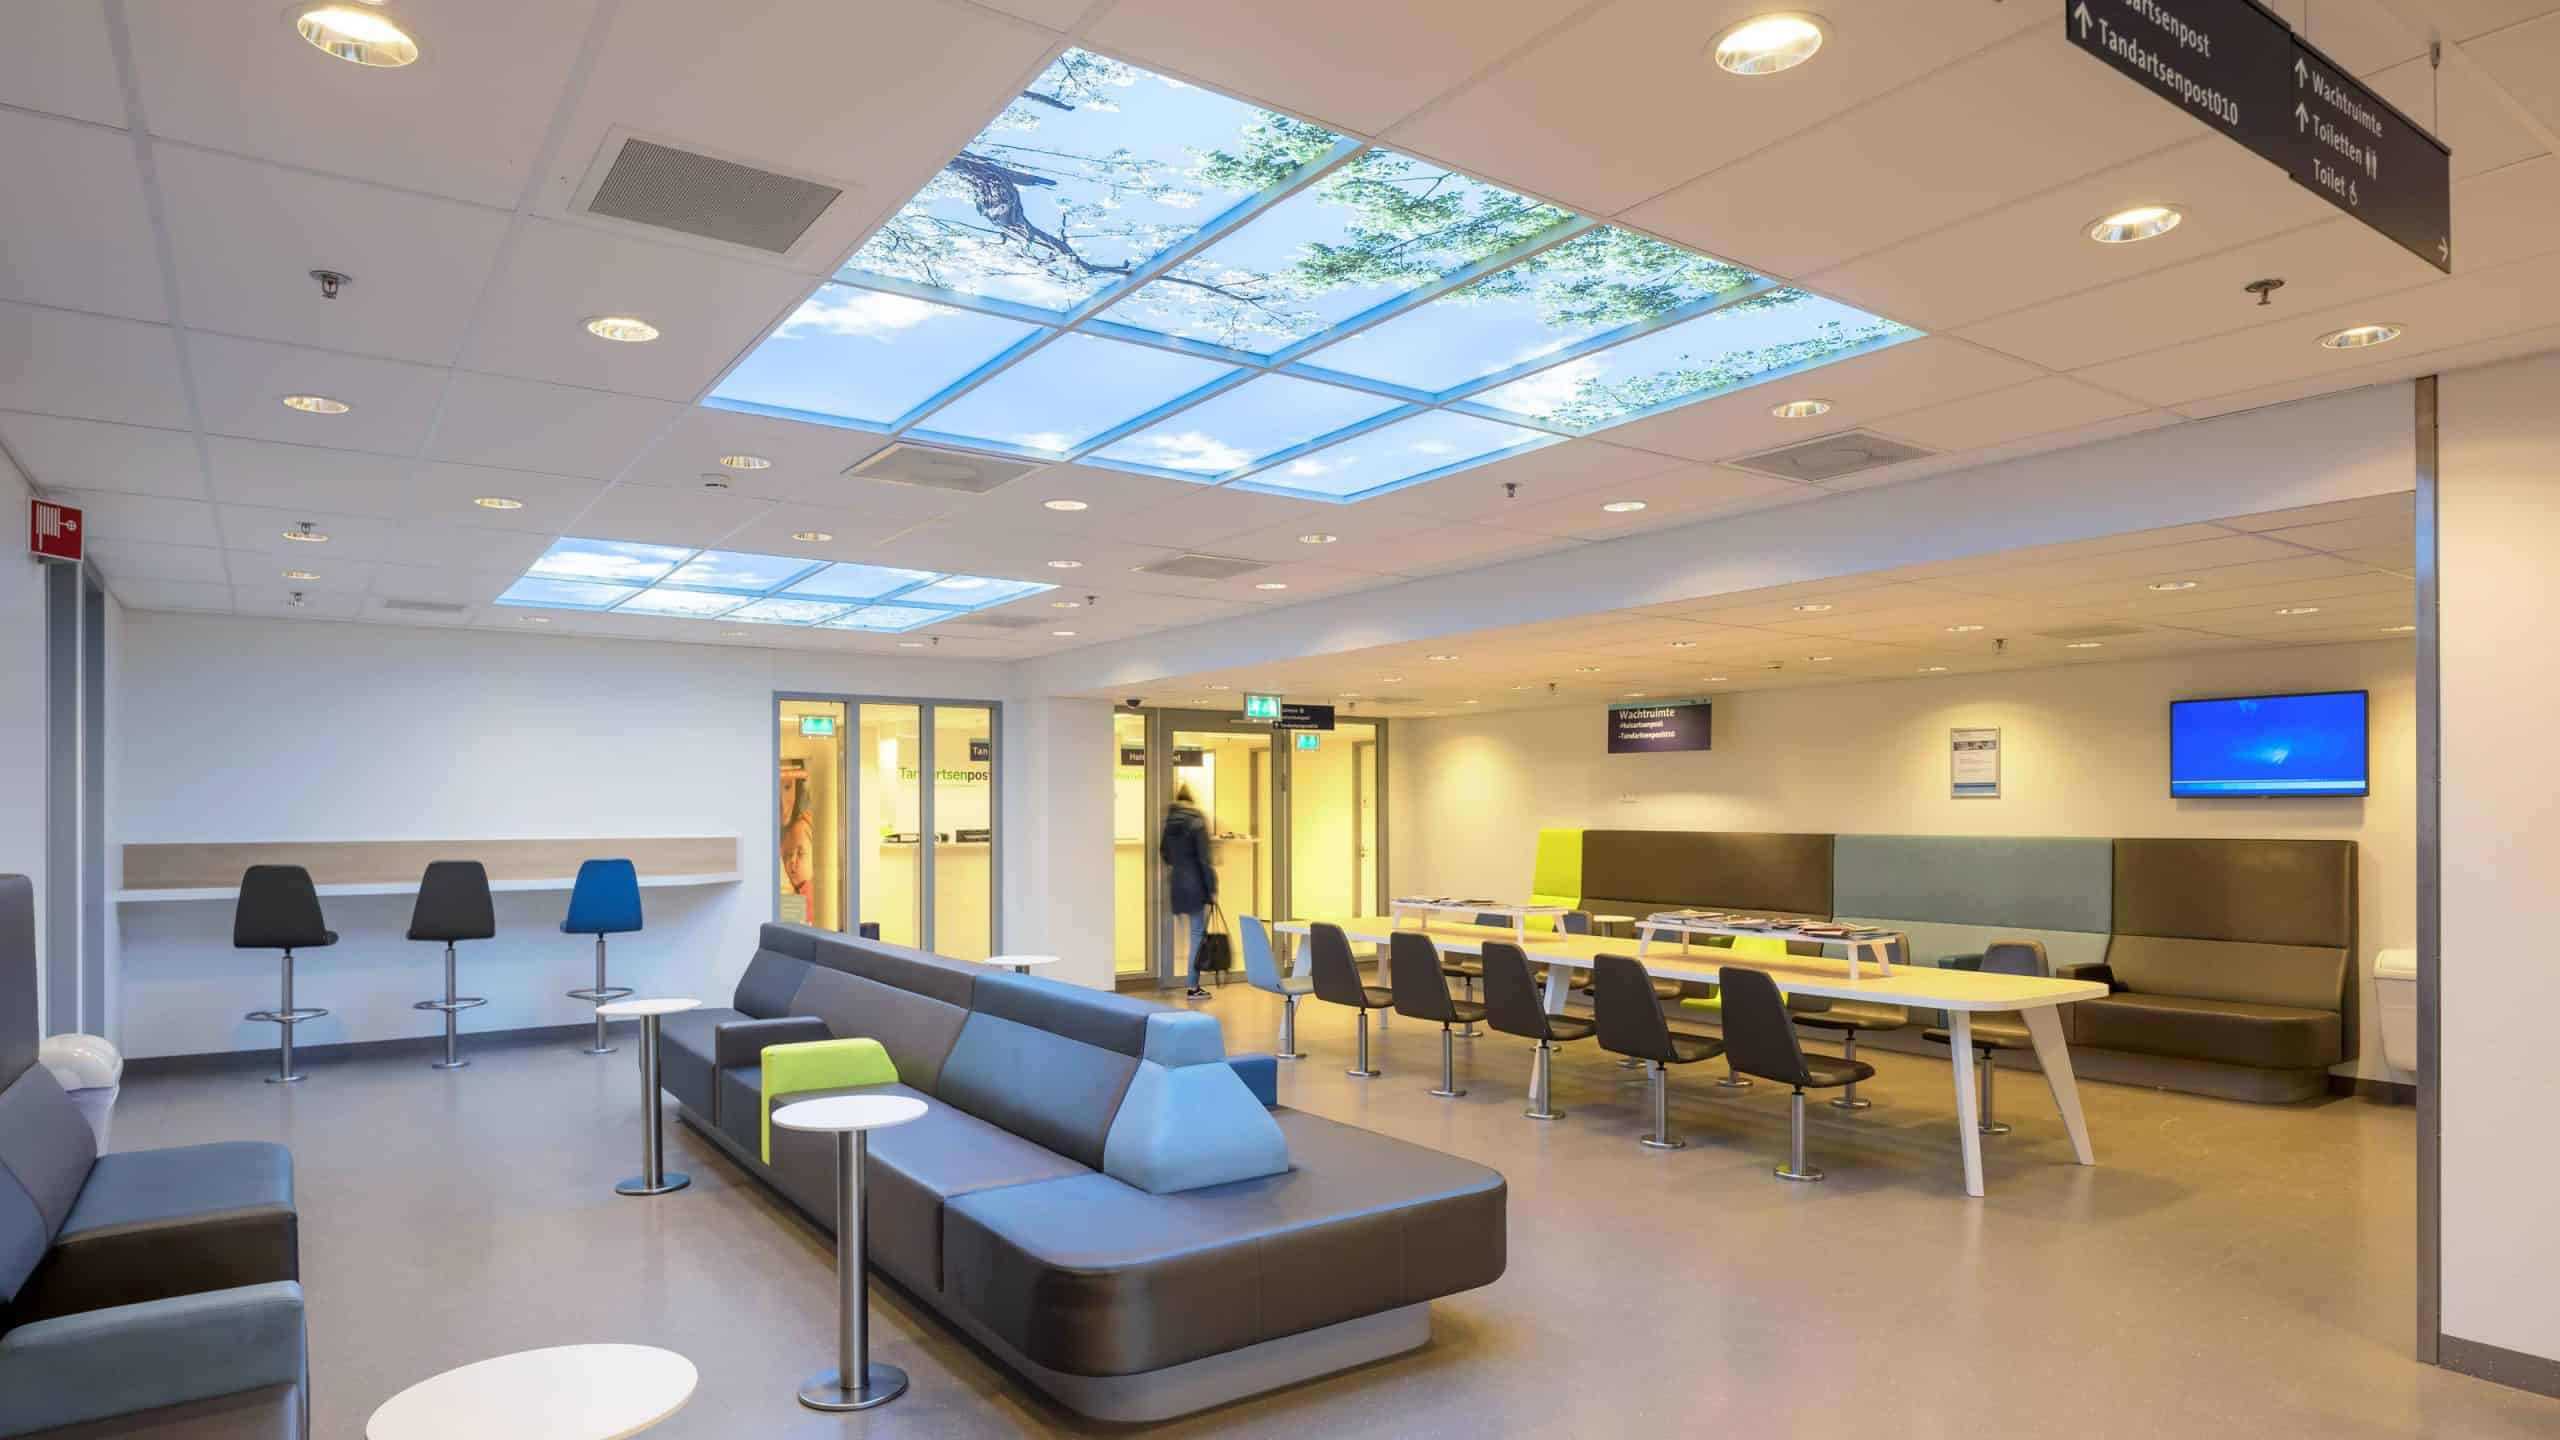
\includegraphics[width=8cm]{img/bp/ziekenhuis.jpg} \\ 
%        \hline
%        Type 2: Mutualiteit en verzekering & Another description for a second type, explaining its use case and characteristics. & 
%        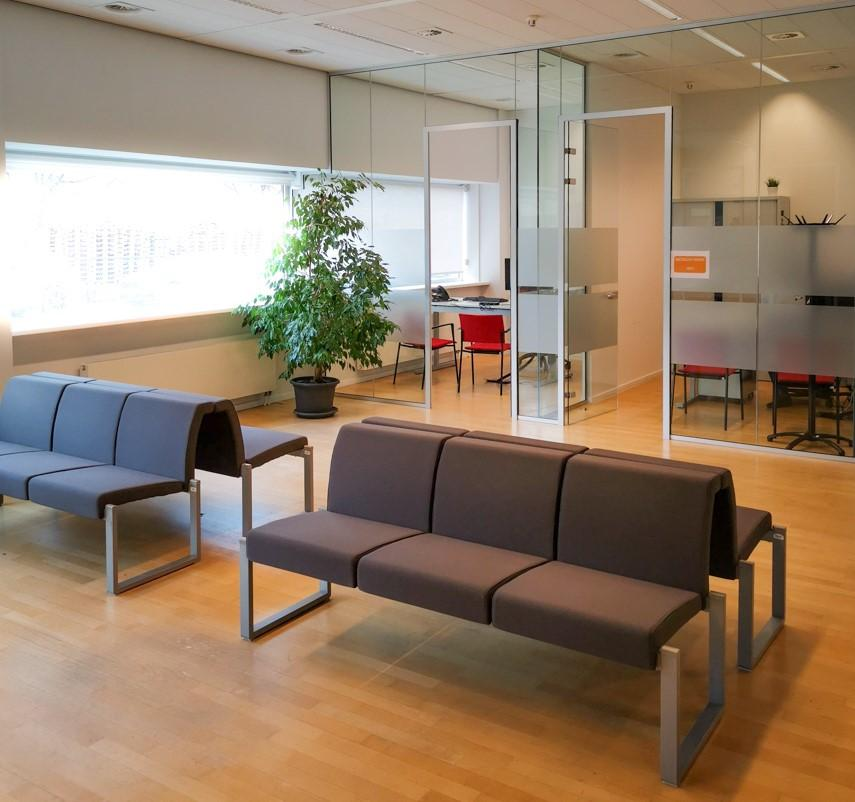
\includegraphics[width=8cm]{img/bp/mutualiteit.jpg} \\ 
%        \hline
%    \end{tabular}
%    \label{tab:type_description_image}
%\end{table}


\section{Selectie van locatie}
Om de Proof-of-Concept uit te voeren is de coöperatie van een medische instelling of andere sectoren noodzakelijk. Naast ziekenhuizen kunnen ook andere zorginstellingen in overweging worden genomen, zoals huisartspraktijken en Woonzorgcentra en Rusthuizen. % voor die reden wordt er naar een ziekenhuis gezocht die met voorkeur in Vlaanderen gelegen is. Het criteria bij het selecteren van een ziekenhuis is de geneigdheid van deze om samen te werken en de beschikbaarheid van de spoedafdeling om de Proof-of-Concept te kunnen uitvoeren. Tot slot moet de spoedafdeling beschikken over een wachtzaal met voldoende capaciteit voor patiënten en benodigde sensoren. 

%Voordat de Proof-of-Concept wordt uitgevoerd, wordt er een ziekenhuis gezocht, bij voorkeur in Vlaanderen. Een ziekenhuis wordt geselecteerd op basis van de bereidheid om samen te werken en de beschikbaarheid van een geschikte spoedafdeling voor het testen van het systeem. De spoedafdeling moet beschikken over een wachtzaal met voldoende capaciteit voor patiënten en benodigde sensoren. Om de samenwerking te vergemakkelijken, kan de Proof-of-Concept worden aangepast zodat deze volledig voldoet aan de geldende GDPR-richtlijnen van het ziekenhuis.
%\section{Locatieanalyse} \label{Locatieanalyse}
%Een grondige locatieanalyse zal uitgevoerd worden om een beter begrip te krijgen over de indeling van de spoedafdeling en wachtruimte. Deze controle wordt verricht om mogelijke obstakels te identificeren, zoals muren en andere structuren. Tijdens de inspectie zal de signaalsterkte gemeten worden door middel van een WiFi site survey software en zullen de toegangspunten voor stroom en netwerken gecontroleerd worden om de beste locatie voor de sensoren te identificeren. Hierbij zal er ook rekening gehouden worden met de locatie van de centrale eenheid en sensorcontroller. Een gedetailleerde kaart zal aangemaakt worden met de optimale locatie van de verschillende componenten. Het uiteindelijke doel van deze sectie is het identificeren van een locatie die de communicatie tussen de verschillende componenten efficiënt laat verlopen. 

\section{Sensoridentificatie en Analyse} \label{sensoridentificatie}
De nodige sensor- en subtypen worden geïdentificeerd door de reeds uitgevoerde literatuurstudie \ref{ch:stand-van-zaken}, die inzicht geeft in welke sensoren kunnen bijdragen bij het realiseren van de proof-of-concept. Deze sensortypes worden geanalyseerd en waar nodig aangevuld met aanvullende bronnen of nieuwe inzichten. De uiteindelijke selectie van sensoren worden geanalyseerd en vergeleken in de vergelijkende studie \ref{vergelijkendeanalyse}, waar de voor- en nadelen van elk type sensor geëvalueerd wordt.

%De reeds geïdentificeerde sensor- en subtypen in de literatuurstudie \ref{ch:stand-van-zaken} worden geanalyseerd en waar nodig aangevuld met aanvullende bronnen of nieuwe inzichten.

%Hierbij zal de huidige literatuurstudie \ref{ch:stand-van-zaken} gebruikt worden bij het analyseren van de reeds identificeerde devices

%daarom wordt er veel aandacht besteed bij het analyseren van de IoT-devices en gebruik hiervan in de gezondheidszorg

%\section{Plaatsingsstrategieën}
%Voor de plaatsing van de sensoren wordt er rekening gehouden met de sectie over plaatsingsstrategieën uit hoofdstuk \ref{ch:stand-van-zaken}. De keuze van de strategie zal afhangen van de resultaten uit de locatieanalyse \ref{Locatieanalyse} Eenmaal de nodige controles uitgevoerd worden de plaatsingsstrategieën uit hoofdstuk \ref{ch:stand-van-zaken} grondig geanalyseerd om de meeste gepaste strategie te implementeren, met als doel om nauwkeurige gegevens te verzamelen.

%\section{Software-identificatie}
%Het identificeren van de software is een belangrijke onderdeel bij het uitvoeren van de Proof-of-Concept. Software is nodig om IoT data te capteren, verwerken, analyseren, visualiseren, filteren en beveiligen. Hierbij is de identificatie van software voor elke stap van het proces essentieel. De identificatie gebeurt door het vaststellen van softwarecomponenten die deel uitmaken van het IoT-systeem. De software wordt geïdentificeerd door gebruik te maken van deze componenten het uitvoeren van een literatuurstudie. De software die hieruit komen worden verder vergeleken in een vergelijkingsstudie \ref{vergelijkingsoftware}.

%\subsection{Identificatie van softwarecomponenten} \label{softwarecomponenten}
%De softwarecomponenten hebben een essentiële rol bij het uitvoeren van de proof-of-concept. Daardoor wordt er aanzienlijk veel tijd besteed aan het identificeren hiervan. De identificatie gebeurt door een analyse van de Proof-of-Concept te realiseren, waarbij diverse componenten worden geïdentificeerd op basis van de benodigdheden van de Proof-of-Concept.

%\subsection{Softwarecomponenten} 
%Voor het identificeren van de softwarecomponenten worden specifieke onderdelen van de proof-of-concept geanalyseerd:

%\begin{table}[h]
%    \tiny
%    \caption{Tabel van de zin uit de PoC en de bijbehorende softwarecomponent}
%    \begin{tabular}{|p{10.5cm}|p{5cm}|}
%        \hline
%        \textbf{Zin uit PoC} & \textbf{Software Component} \\ \hline
%        De centrale eenheid of solution in de cloud verwerkt deze gegevens en berekent de volgorde en wachttijden van patiënten in de wachtruimte op basis van de tijdstempels. & Data Verwerking en Analyse \\ \hline
%        De data kan in real-time worden geanalyseerd om de wachttijden te berekenen en om te bepalen welke patiënt als volgende aan de beurt is. & Data Verwerking en Analyse \\ \hline
     %   Om de kans op false-positives en onnauwkeurige data te minimaliseren, worden technieken zoals filtering (om ruis te verminderen) en debouncing (om fluctuaties in digitale signalen te stabiliseren) toegepast op de sensorgegevens. & Debouncing en filtering van sensor data \\ \hline
        %Het dashboard zorgt ervoor dat het personeel gedetailleerde informatie kan raadplegen over de wachtruimte zoals het aantal patiënten, geschatte wachttijd per patiënt en volgorde van behandeling. & Dashboard en Visualisatie \\ \hline
        %De verzamelde data wordt vervolgens verstuurd door de sensor controller naar de centrale eenheid via een seriële verbinding of draadloze protocol & Netwerk en communicatieprotocol \\ \hline
%        Een thermische camera zal tot slot gebruikt worden om staande patiënten te detecteren & Integratie voor een thermische camera \\ \hline
        %Aangezien dat IoT-technologieën diverse beveiligings- en ethische risico's met zich meebrengen worden er verschillende beveiligings- en ethische maatregelen geïmplementeerd zelfs als er geen persoonlijke gegevens verzameld worden. & Gegevensbeveiliging \\ \hline
%    \end{tabular}
%    \label{tab:zin_software}
%\end{table}

%\begin{itemize}
    %\item \textbf{IoT Hardware-software:} Software voor het beheren van de sensoren die de beweging en aanwezigheid van patiënten detecteren.
%    \item \textbf{Data Verwerking en Analyse:} Voor het verwerken van sensorgegevens en het analyseren hiervan.
    %\item \textbf{Dashboard en Visualisatie:} Software voor het visualiseren van de verwerkte gegevens.
    %\item \textbf{Debouncing en filtering van sensor data:} Software voor het verminderen van ruis en stabiliseren van digitale signalen.
    %\item \textbf{Netwerk en communicatieprotocol:} Software voor de communicatie tussen de sensoren, sensorcontroller en centrale eenheid.
    %\item \textbf{Gegevensbeveiliging:} Software voor mogelijke gegevensbeveiliging indien nodig.
%    \item \textbf{Integratie voor een thermische camera} Software voor de integratie van een thermische camera.
%\end{itemize}

%Na het identificeren van de software worden deze voor elke implementatie met elkaar vergeleken in een vergelijkende studie \ref{vergelijkendeanalyse}.

%\section{Identificatie van een cloud oplossing} \label{cloud}
%Bij het uitvoeren van de Proof-of-Concept zal er gebruik gemaakt worden van een cloudgebaseerd platform. Hierop zal een software draaien die verantwoordelijk is voor het analyseren van de binnenkomende data en de wachttijden berekenen. Net zoals bij de selectie van IoT devices en identificeren van software zal er gebruik gemaakt worden van een vergelijkende studie waarbij diverse cloud oplossingen vergeleken worden op basis van de volgende kenmerken

%\section{Case study}
%Deze case study heeft als hoofddoel het verklaren van de implementatie van IoT technologieën door het identificeren van concrete voorbeelden van IoT-gebruik bij het verminderen van wachttijden op A\&E afdelingen. De case study richt zich verder op het vaststellen van IoT apparaten die ingezet kunnen worden om wachttijden te verkorten. De case study begint met het identificeren van specifieke casussen. Hiervoor worden verschillende bronnen geraadpleegd (Academische artikelen, Boeken, Wetenschappelijke artikelen, enzovoort) met als doel om kwalitatieve en kwantitatieve gegevens te verzamelen. De IoT-devices en categorieën die voorkomen in de casussen worden verder opgelijst en geanalyseerd. Tot slot worden verschillende bronnen geraadpleegd bij het verzamelen van gegevens voor iedere identificeerde IoT-device. Deze gegevens zullen verder in de volgende fase gebruikt worden.

%Deze case study wordt uitgevoerd als toelichting voor het implementeren van IoT technologieën. De primaire doelstelling van deze case study is het identificeren van praktische voorbeelden van IoT gebruik om lange wachttijden in A\&E afdelingen te verminderen. Daarnaast richt de case study zich op het identificeren van verschillende IoT apparaten die ingezet kunnen worden om wachttijden verder te verkorten. De case study begint met het identificeren van specifieke casussen. Na het vaststellen van een casus worden er kwalitatieve en kwantitatieve gegevens verzameld over de gekozen casus, dit houdt in dat verschillende bronnen worden geraadpleegd bij het verzamelen van informatie zoals wetenschappelijke literatuur, rapporten van gezondheidsorganisaties, archieven en documenten. Na het vaststellen van diverse casussen worden deze geanalyseerd en de gebruikte IoT-devices en IoT categorieën opgelijst. Verder worden gegevens verzameld voor elk van de opgelijste devices, verschillende bronnen zoals onderzoeksrapporten, literatuurstudies, academische tijdschriften en technologische onderzoeken worden hiervoor geraadpleegd. 

%\section{Identificeren van IoT-devices}
%Het identificeren van IoT-devices is een essentiële fase in deze studie, daarom wordt er veel aandacht besteed bij het uitwerken van de case study en bijgevolg het identificeren van IoT-devices. Deze devices worden geselecteerd op basis van de categorie waartoe ze behoren. De categorieën worden bepaald volgens de benodigdheden in van de proof-of-concept. Elke device die tot een categorie behoort wordt grondig bestudeerd om beter te begrijpen hoe deze werkt en geïmplementeerd kan worden in de proof-of-concept. \ASK

%Het identificeren van IoT apparaten is van het uiterste belang, daarom is er aanzienlijk veel tijd besteed aan het opstellen van de casestudie om een assortiment van IoT apparaten te bepalen. Dit houdt in dat elk device grondig bestudeerd zal worden om een beter begrip te krijgen in de werking hiervan in de gezondheidszorg. Om het meest gepaste IoT device te selecteren worden verschillende IoT categorieën bekeken, deze categorieën vertegenwoordigen IoT apparaten die de werking van de A\&E afdelingen kunnen verbeteren en efficiënter maken, deze categorieën zijn: Locatie- en traceerapparaten, Communicatieapparaten, Integratie van het gegevensbeheer en Integratie en coördinatie van IoT devices. De categorieën worden geselecteerd op basis van de nodige IoT devices in de proof-of-concept. Het Real-time Smart Queue Management System maakt gebruik van bewegings- en aanwezigheidssensoren, die worden ingezet om de locatie van patiënten in de wachtrij in real-time te volgen.

\section{Vergelijkende analyse} \label{vergelijkendeanalyse}
In deze sectie wordt een vergelijkende studies uitgevoerd over de IoT devices. Het doel van deze studies is om de meest geschikte devices te identificeren voor de proof-of-concept.

\subsection{Vergelijkende studie: IoT-devices}
Om de meest gepaste IoT device(s) te selecteren voor het uitvoeren van de proof-of-concept is het noodzakelijk om de verschillende apparaten met elkaar te vergelijken. om voor de hand liggende redenen worden de apparaten eerst vergeleken op de voor- en nadelen die deze brengen. Verder door dat het budget gelimiteerd is wordt er rekening gehouden met de aanschafkosten van de apparaten.

%\subsubsection{Inhoud vergelijkende studie: IoT devices}
%De vergelijkende studie bevat de volgende criteriums:
%\begin{itemize}
%    \item \textbf{Voor- en nadelen:} Een overzicht van de voordelen en nadelen van elk apparaat.
%    \item \textbf{Kosten:} De kostenanalyse omvat enkel de aanschafkosten.    
    %\item \textbf{Betrouwbaarheid:} Hier wordt gekeken naar de stabiliteit van het apparaat, de kwaliteit van de hardware.    
    %\item \textbf{Gebruiksvriendelijkheid:} Dit criterium omvat de eenvoud van installatie, configuratie, bediening.    
    %\item \textbf{Integratie capaciteit:} De mogelijkheid om het IoT apparaat te integreren met andere systemen of apparaten (Raspberry Pi, Arduino) wordt onderzocht. 
%\end{itemize}

\subsubsection{Devices}
In deze vergelijkende studie worden verschillende types devices met elkaar vergeleken die nodig zijn bij de implementatie van de proof-of-concept. Het identificeren van de devices gebeurt door het raadplegen van de uitgevoerde literatuurstudie en bijkomende onderzoeken. devices worden geïdentificeerd voor de volgende componenten.

\begin{itemize}
    \item Centrale eenheid
    \item Sensor controller
    \item Lichtsluis/IR-sensor
    \item PIR-bewegingssensoren
    \item Ultrasoon/infraroodsensoren
    %\item CO₂ Sensor (Detectie van  CO₂ levels)
\end{itemize}


\subsubsection{Methodologie van vergelijking}

De vergelijkende studie bevat de volgende criteriums:
\begin{itemize}
    \item \textbf{Centrale eenheid en sensor controller}
    \begin{itemize}
        \item Voor- en nadelen: Een overzicht van de voordelen en nadelen van deze twee componenten.
        \item Kosten: De kostenanalyse omvat enkel de aanschafkosten van deze onderdelen.  
    \end{itemize}
    
    \item \textbf{Lichtsluis/infraroodsensoren}
    \begin{itemize}
        \item Nauwkeurigheid
        \item Connectiviteit
        \item Kost (€)
    \end{itemize}

    \item \textbf{PIR-bewegingssensoren}
    \begin{itemize}
        \item Gevoeligheid
        \item Nauwkeurigheid
        \item Kost (€)
    \end{itemize}
    
    \item \textbf{Ultrasoon/infraroodsensoren}
    \begin{itemize}
        \item Bereik
        \item Nauwkeurigheid
        \item Kost (€)
    \end{itemize}

        
    %\item \textbf{Betrouwbaarheid:} Hier wordt gekeken naar de stabiliteit van het apparaat, de kwaliteit van de hardware.    
    %\item \textbf{Gebruiksvriendelijkheid:} Dit criterium omvat de eenvoud van installatie, configuratie, bediening.    
    %\item \textbf{Integratie capaciteit:} De mogelijkheid om het IoT apparaat te integreren met andere systemen of apparaten (Raspberry Pi, Arduino) wordt onderzocht. 
\end{itemize}

\subsubsection{Vergelijking van devices}

\begin{table}[h!]
    \tiny
    \caption{Vergelijking van Centrale Eenheden voor IoT \autocite{Calvo2016, Hosny2023, SainzRaso2019, 王丁2014, Pham2024, Chatterjee2022}}
    \label{tab:vergelijking-centrale-eenheid}
    \begin{tabular}{|p{1.5cm}|p{3.5cm}|p{3.5cm}|p{3.5cm}|}
        \hline
        \textbf{Criteria} & \textbf{Raspberry Pi} & \textbf{HP EliteDesk 800 G3 USFF} & \textbf{NVIDIA Jetson Nano} \\
        \hline
        \textbf{Voordelen} & Betaalbaar, gemeenschapsbreed gesteund, ideaal voor kleinere IoT-projecten & Compact en energie-efficiënt design, geschikt voor kleine werkruimtes & Krachtig voor real-time verwerking, energiezuinig, ideaal voor mobiele toepassingen \\
        \hline
        \textbf{Nadelen} & Beperkingen in CPU, RAM, kwetsbaar door afhankelijkheid van software en OS & Beperkingen in rekenkracht, problemen met koeling en connectiviteit & Beperkingen in geheugen en rekenkracht voor grotere AI-modellen, niet geschikt voor zware GPU-taken  \\
        \hline
        \textbf{Kost (€)} & IN BEZIT & €99,00 & €200-300 \\
        \hline
    \end{tabular}
\end{table}

%---------------------------------------------------------------------------------------------

\begin{table}[h]
    \tiny
    \caption{Vergelijking van Sensor Controllers \autocite{Hussain2024, Viriyavisuthisakul2017, Spohn2020, Maier2017, Wang2020, Wu2020, Kovacshazy2024}}
    \label{tab:vergelijking-sensorcontroller}
    \begin{tabular}{|p{1.5cm}|p{3.5cm}|p{3.5cm}|p{3.5cm}|}
        \hline
        \textbf{Criteria} & \textbf{Arduino Nano 33 IoT} & \textbf{ESP32-WROOM} & \textbf{STM32} \\
        \hline
        \textbf{Voordelen} 
        & Kosteneffectief. In retail detecteert het wachtrijlengtes en waarschuwt personeel. 
        & Efficiënt voor IoT met laag verbruik, dual-core en WiFi/Bluetooth. 
        & Hoge performantie en energie-efficiëntie in uiteenlopende IoT-toepassingen. \\
        \hline
        \textbf{Nadelen} 
        & Beperkte kracht en geen RTOS, lastig voor complexe toepassingen. 
        & Lagere performantie bij hoge zendfrequenties en druk WiFi-netwerk. 
        & Uitdagingen bij toepassingen met hoge verwerkingsvereisten en complexe connectiviteit. \\
        \hline
        \textbf{Kost (€)} 
        & €28,07 
        & €19,95 
        & €24,13 \\
        \hline
    \end{tabular}
\end{table}


%----------------------------------------------------------------------------------------------
\begin{table}[h!]
    \tiny
    \caption{Vergelijking van Lichtsluis-infraroodsensoren \autocite{}}
    \begin{tabular}{|p{3.5cm}|p{3cm}|p{3cm}|p{3cm}|}
        \hline
        \textbf{Feature} & \textbf{Sharp GP2Y0A21YK0F} & \textbf{TCS3200 TCS230} & \textbf{Adafruit TSL2561} \\
        \hline
        \text{Meetmethode} & Infrarood afstand & Optisch (RGB-kleur detectie) & Lichtsensor (Lux meeteenheid) \\
        \hline
        \text{Bereik} & 10 - 80 cm & 0 - 2 meter & 0 - 100,000 Lux \\
        \hline
        \text{Kost (€)} & €36.19 & €36.29 & €73.95 \\
        \hline
    \end{tabular}
\end{table}




%----------------------------------------------------------------------------------------------
\begin{table}[h]
    \tiny
    \caption{Vergelijking van PIR-bewegingssensoren \autocite{Wellue2025, Zacurate2025, Jumper2025}}
    \label{tab:vergelijking-thermische-camera}
    \begin{tabular}{|p{3cm}|p{3.5cm}|p{4.5cm}|p{3.5cm}|}
        \hline
        \textbf{Criterium} & \textbf{HC-SR501} & \textbf{AM312} & \textbf{RCWL-0516} \\
        \hline
        Bereik & 7 meter & 3 meter & 5-8 meter \\
        \hline
        Detectiehoek & 120° & 70° & 360° \\
        \hline
        Kost (€) & €5,95 & €2,25 & €1.80 \\
        \hline
    \end{tabular}
\end{table}


%----------------------------------------------------------------------------------------------
\begin{table}[h]
    \tiny
    \caption{Vergelijking van Ultrasoon/Infraroodsensoren \autocite{Acconeer2023, Acconeer2023a, Infineon2024}}
    \label{tab:vergelijking-pressure-sensor}
    \begin{tabular}{|p{2.5cm}|p{2.5cm}|p{4.7cm}|p{5.5cm}|}
        \hline
        \textbf{Criterium} & \textbf{HC-SR04} & \textbf{Parallax Inc PING} & \textbf{MB1240 XL-MaxSonar-EZ4} \\
        \hline
        Bereik & 2cm - 4m & 2 cm - 3 m & 20cm - 7m \\
        \hline
        Nauwkeurigheid & ±0.3 cm & ±1 cm & ±1 cm \\
        \hline
        Kosten (€) & €2,10 & €33,11 & €29,95 \\
        \hline
    \end{tabular}
\end{table}



\subsubsection{Conclusie vergelijkende studie}
Volgens de bevindingen  uit de vergelijkende studie worden de volgende devices geselecteerd voor implementatie in de proof-of-concept.

\begin{table}[h]
    \tiny
    \renewcommand{\arraystretch}{1.2}
    \caption{Geselecteerde IoT Devices}
    \begin{tabular}{|l|c|p{9cm}|}
        \hline
        \textbf{IoT Device} & \textbf{Price (EUR)} & \textbf{Reason of Choice} \\
        \hline
        Raspberry Pi & IN BEZIT & Reeds in bezit, veelzijdig voor prototyping. De beveiligingsnadelen zijn voor de PoC minder van belang.\\
        ESP32-WROOM & €19,95  & Kost, Laag energieverbruikt, dual-core en Wi-Fi Bluetooth support. \\
        MLX90614  & €17,99 & Nauwkeurig, snel, goedkoop \\
        Zacurate Pro Series 500DL & €35,65  & Betrouwbaar, goedkoop \\
        Infineon XENSIV BGT60TR13C & €9,59  & Compact, accuraat, kostenefficiënt \\
        \hline
        \textbf{Total} & \textbf{€83,18} & \\
        \hline
    \end{tabular}
    \label{tab:iot_prices}
    \end{table}}


%--------------------------------------------------------------------------------------------
%\subsection{Vergelijkende studie: Cloudgebaseerde platform}
\TODO


%--------------------------------------------------------------------------------------------
%\subsection{Vergelijkende studie: Software componenten} \label{vergelijkingsoftware}
%In deze sectie worden verschillende software componenten met elkaar vergeleken om de meest geschikte keuze te maken voor de Proof-of-Concept. De resultaten van deze vergelijking leiden tot een aanbeveling voor de meest geschikte softwarecomponent voor de Proof-of-Concept. Deze aanbeveling wordt ondersteund door een uitgebreide uitleg van waarom bepaalde software de voorkeur krijgen boven andere, met speciale aandacht voor hoe ze bijdragen aan de doelstellingen van het project.

%\subsubsection{Keuze methodologie van vergelijking}
%Voor een objectieve vergelijking wordt diverse vergelijkingsmethodologieën onderzocht, hiervoor worden verschillende website(s) geraadpleegd zoals wetenschappelijke studies en onafhankelijke reviewplatformen zoals Gartner, Capterra en Trustradius. Daarnaast worden academische studies geanalyseerd om de meest gepaste methode te selecteren voor elke criteria. Een methodologie wordt verder geselecteerd op basis van de soort van gegeven (kwantitatief, kwalitatief).

%\subsubsection{Inhoud vergelijkende studie: Softwarecomponenten}
%De softwarecomponenten die vergeleken worden zijn benoemd onder sectie \ref{softwarecomponenten} \textit{Identificatie van software componenten}. 

%\subsubsection{Vergelijkingscriteria}
%Om een duidelijke beeld te krijgen over de meest geschikte software worden deze op diverse kwantitatieve en kwalitatieve criteria vergeleken. Deze criteriums dekken belangrijke aspecten van zowel de technische en operationele kant van softwaretoepassingen.

%\begin{itemize}
%    \item \textbf{Kosten:} De kostenanalyse omvat zowel de licentiekosten als eventuele implementatie- en onderhoudskosten, voor de implementatiekosten wordt er rekening gehouden met kosten voor cloudgebaseerd platformen. \TODO
%    \item \textbf{Betrouwbaarheid:} De stabiliteit van de software wordt geëvalueerd op basis van throughput, Latency en fault tolerance.
%    \item \textbf{Ondersteuning en community:} De beschikbaarheid van documentatie en ondersteuning. 
%    \item \textbf{Gebruiksvriendelijkheid:} Dit criterium omvat de eenvoud van installatie, configuratie en het gebruik van de software.
%    \item \textbf{Integratiemogelijkheden:} De mogelijkheid om de softwarecomponent te integreren met andere systemen of platforms (zoals databases, IoT-apparaten, API’s) wordt onderzocht. 
%\end{itemize}

%\subsubsection{Vergelijkingsmethodologieën}

%\begin{table}[h]
%    \caption{Overzicht van methodologieën per criterium}
%    \centering
%    \tiny
%    \renewcommand{\arraystretch}{1.3}
%    \begin{tabular}{|p{4cm}|p{5cm}|p{6cm}|}
%        \hline
%        \textbf{Criterium} & \textbf{Methodologie} & \textbf{Toelichting} \\ \hline
%        Kosten & TCO-analyse (Total Cost of Ownership) & Vergelijking van licentie, hostingkosten. \\ \hline
%        Betrouwbaarheid & Empirische analyse + SLA-analyse & Betrouwbaarheid wordt gemeten met historische gegevens, statistieken en Service Level Agreements (SLA) \\ \hline
%        Ondersteuning en community & Benchmarking & Vergelijk, responsiviteit van de community en beschikbaarheid van technische ondersteuning. \\ \hline
%        Gebruiksvriendelijkheid & Usability Testing & Uittesten van de software en beoordeel op basis van gebruiksvriendelijkheid. \\ \hline
%        Integratiemogelijkheden & Feature-matching + API-documentatieanalyse & Onderzoek compatibiliteit met andere systemen en de flexibiliteit van API’s. \\ \hline
%    \end{tabular}
%    \label{tab:methodologieen}
%\end{table}


%\subsubsection{Vergelijking van softwarecomponenten}

%\paragraph{Kosten}
%\TODO

%\paragraph{Betrouwbaarheid}
%De betrouwbaarheid wordt gemeten dankzij een empirische- en SLA analyse. De meting wordt uitgevoerd op basis van de volgende metrieken: 

%\begin{table}[ht]
%    \tiny
%    \caption{Evaluatie van de stabiliteit van de software, \autocite{Padmanaban2024, Raza2021, Singh2022, Rinaldi2019, Mehdi2023, Chakraborty2021, Rajput2024}}
%    \renewcommand{\arraystretch}{1.5} % Verhoog de rijhoogte voor meer ruimte
%    \begin{tabular}{|l|l|p{5cm}|p{4cm}|p{4cm}|} % Extra kolom voor categorie
%        \hline
%        \textbf{Categorie} & \textbf{Software} & \textbf{Throughput} & \textbf{Latency} & \textbf{Fault tolerance} \\
%        \hline
%        Verwerking & Apache Kafka & 750-1340 events per uur. & 6-15 milliseconden & Er bestaat fout tolerantie voor netwerk problemen maar er zijn tekorten.  \\
%        \hline
%        Analyse & Apache Flink & +1 miljoen events per seconde & 2.5-2.7 milliseconden voor complexe queries & Heeft een robuuste fouttolerantie, deze heeft een impact op de performantie maar is essentieel voor de betrouwbaarheid.  \\
%        \hline
%        Verwerking & InfluxDB & Kan variëren van millisecondes naar secondes volgens de data model. & 3.374 milliseconden & Er bestaat fout tolerantie. \\
%        \hline
%        \textbf{Categorie} & \textbf{Software} & \textbf{Ease of use} & \textbf{Best for} & \textbf{Data Connectivity} \\
%        \hline
%        Monitoring & Grafana & Gebruiksvriendelijk interface maakt het gebruik makkelijk voor gebruikers met verschillende technische achtergronden. Dit maakt het configureren, aanpassen en visualiseren makkelijk  & Real-time monitoring en visualiseren van data uit verschillende bronnen. Grafana is uitstekend bij het creëren van interactieve aanpasbare dashboards dat data van servers, databases en IoT devices integreert. & Ondersteunt diverse time-series en SQL-databases. \\
%        \hline
%        Monitoring & Power Bi & Gebruikersvriendelijk dankzij zijn drag-and-drop interface & N/A & N/A \\
%        \hline
%        Monitoring & Tableau & De bevindingen tonen de snelheid en effectiviteit van de technische ondersteuning bij het oplossen van problemen, met een gemiddelde oplostijd van 4 uur. & N/A & N/A \\
%        \hline
%    \end{tabular}
%\end{table}


%\subsubsection{Resultaten en Discussie}

%\subsubsection{Conclusie en aanbevelingen}
%-----------------------------------------------------------------------------------------------

\section{Procedure: Proof-of-Concept (PoC)}
De Proof-of-Concept (PoC) onderzoekt hoe IoT-technologie kan worden ingezet om wachttijden bij Solidaris Ronse in kaart te brengen, transparant te maken en uiteindelijk te verkorten.

\subsection{Nulmeting en verzameling van historische gegevens}
Om de effectiviteit van het Proof-of-Concept (PoC) te evalueren, wordt eerst een nulmeting uitgevoerd tijdens een piekmoment. Hierbij wordt gebruikgemaakt van een tool (Google Occupancy Rate API, OpenCV) om de huidige bezettingsgraad van de wachtruimte te meten. Tijdens deze meting worden gegevens verzameld zoals het aantal aanwezigen per tijdseenheid, het verloop van piek- en dalmomenten en indien mogelijk de gemiddelde wachttijden. Deze gegevens vormen de baseline waarmee achteraf de impact van het nieuwe IoT-gebaseerde systeem objectief kan worden beoordeeld.

\subsection{Opbouw van het meetsysteem}
In het Proof of Concept (PoC) wordt een eenvoudige IoT-architectuur gebruikt waarbij sensoren in real-time registreren hoeveel mensen aanwezig zijn. De metingen gebeuren volledig anoniem, zonder tracking op persoonsniveau. De verzamelde gegevens worden automatisch doorgestuurd naar een relationele database voor opslag. 

\subsection{Technische uitwerking}
Het meetsysteem in deze Proof-of-Concept maakt gebruik van verschillende sensortechnologieën die anoniem de aanwezigheid en beweging van patiënten in de wachtruimte registreren. Sensoren worden ingezet om de bewegingen van personen binnen de ruimte te detecteren. Aan de ingangen en doorgangen worden sensoren geplaatst voor het nauwkeurig detecteren of iemand een ruimte binnenkomt of verlaat en in welke richting, wat essentieel is om dubbele tellingen te voorkomen. Daarnaast wordt een type sensoren gebruikt om afstanden tot personen te meten. Dit laat toe om ook personen te detecteren, ongeacht of ze staan of zitten, zelfs als zij weinig tot geen beweging vertonen. Door deze sensoren te combineren ontstaat een betrouwbaar beeld van de actuele bezetting, zonder gebruik te maken van camera’s of persoonsgegevens. Alle metingen gebeuren dus volledig privacyvriendelijk en in real-time, waardoor het systeem geschikt is voor toepassing zoals een wachtzaal van een mutualiteit zoals Solidaris.

\subsection{Little's Law-formule}
Little's Law is één van de meest gebruikte wet bij het bestuderen en optimaliseren van wachttijden.

\[
L = \lambda W
\]

Uitleg:
\begin{itemize}
    \item \( L \) Is de gemiddelde aantal personen in het systeem.
    \item \( \lambda \) is de aankomstsnelheid (het gemiddelde aantal personen dat per tijdseenheid aankomt).
    \item \( W \) is de gemiddelde tijd die een item in het systeem doorbrengt.
\end{itemize}

\subsection{Validatie van bezettingsmetingen}
Vooraleer de verzamelde gegevens worden gebruikt voor verdere analyse, wordt gecontroleerd of het meetsysteem correcte en consistente resultaten oplevert. Dit gebeurt via steekproeven waarbij het aantal aanwezigen in de wachtruimte handmatig wordt geteld en vergeleken met de waarden die automatisch door het systeem zijn geregistreerd. Indien afwijkingen worden vastgesteld, wordt het systeem aangepast of opnieuw gekalibreerd. Deze validatie garandeert de betrouwbaarheid van de data voor latere vergelijking met de nulmeting.

\subsection{Verwerking en vergelijking van gegevens}
De resultaten van het IoT-gebaseerde wachttijdbeheersysteem worden vergeleken met de resultaten uit de nulmeting op basis van de bezettingsgraad. Deze vergelijking maakt het mogelijk om objectief te evalueren of het gebruik van IoT-technologie daadwerkelijk leidt tot een vermindering van wachttijden en een efficiënter bezoekersbeheer.

%\subsection{Realtime feedback en optimalisatie}
%Dankzij de real-time gegevens kan het systeem bijdragen aan wachttijdreductie door het bezoekerscomfort te verhogen, doordat bezoekers via een website kunnen zien wanneer het minder druk is en zo hun bezoek beter kunnen plannen. Daarnaast maakt het systeem druktevoorspelling mogelijk: naarmate er meer historische data beschikbaar is, kunnen verwachte drukke momenten steeds nauwkeuriger voorspeld worden.

\subsection{Voorspellende analyses}
Op basis van de verzamelde historische gegevens wordt een voorspellend model ontwikkeld. Dit model kan trends en patronen in bezoekersgedrag identificeren, zoals typische piekmomenten per dag of week. Door deze voorspellingen kunnen bezoekers en personeel zich beter voorbereiden op verwachte drukte, wat de wachttijdreductie verder ondersteunt. 

\subsection{Hoe IoT concreet bijdraagt aan wachttijdreductie}
De verzamelde gegevens maken real-time optimalisatie mogelijk doordat het systeem drukke momenten kan voorspellen en zo bijdraagt aan beter personeelsbeheer. Bovendien draagt het systeem bij aan een efficiënter bezoekersbeheer, waardoor de wachttijden beter te voorspellen zijn en bezoekers hun tijd optimaler kunnen benutten.


%Iedere patiënt krijgt een triage niveau, dit zorgt ervoor dat patiënten met kritische triage niveau prioriteit krijgen.
%Door de patiënten te triëren volgens diverse triage niveaus kunnen patiënten sneller behandeld worden. 
%De wachttijden die verzameld worden door de diverse IoT-devices kunnen verder gebruikt worden om de responsiviteit te verhogen en zo de wachttijden te verkorten. Dit wil zeggen dat in geval van hoge wachttijden dit een teken kan zijn om extra registratiemedewerkers of triagepersoneel in te zetten. Het tijdelijk verhogen van de personeel bij lange wachttijden kan ervoor zorgen dat de doorstroming van patiënten versneld wordt, waardoor de totale wachttijd afneemt. Historische data samen met de real-time metingen kunnen gebruikt worden voor het herkennen van trends zoals terugkerende piekmomenten op bepaalde tijdstippen of dagen. Dit maakt het mogelijk om personeel beter in te zetten door proactief in te plannen voor drukke periodes, zodat er altijd voldoende personeel beschikbaar is wanneer dat nodig is.



%\subsection{Aankomst van de patiënt op de afdeling}
%Het onderzoek begint met het verzamelen van de wachttijden van de binnenkomende patiënten. Het is hierbij belangrijk dat de spoedeisende patiënt niet weet dat hij deelneemt aan het onderzoek om onnodige zorgen te voorkomen. Dit is echter mogelijk dankzij de grootte van de devices en het implementeren hiervan op een discrete manier zodat patiënten er niet van bewust zijn dat het wachttijden gemeten wordt. Het meten begint wanneer een patiënt de ruimte binnentreedt. Een emitter- en een receiver-sensor worden aan beide zijden van de ingang geïnstalleerd. De emitter zendt een infraroodstraal naar de receiver, en wanneer de straal wordt onderbroken, activeert dit de sensor, die vervolgens een tijdstempel registreert. Om aan de privacy-richtlijnen te voldoen worden geen gegevens verzameld, maar om toch de patiënten te kunnen differentiëren wordt er een Unique Identifier (UID) toegekend aan iedere patiënt. 



%\section{Impactanalyse}
%De impactanalyse heeft als doel om te onderzoeken welke impact de proof-of-concept inclusief de geselecteerde devices zal hebben op de spoedafdeling.

%\subsection{Inhoud impactanalyse} 
%\begin{itemize}
%    \item \textbf{Doelen en verwachte resultaten:} Een gedetailleerde overzicht over wat er bereikt zal worden met de proof-of-concept.
    
%    \item \textbf{Kosten:} Analyse van de financiële impact van de implementatie zoals de kosten van sensoren, cloud, onderhoudskosten, enz...
    
%    \item \textbf{Impact op belanghebbenden} Het beoordelen van de impact van het systeem op patiënten, zorgverleners en ziekenhuispersoneel.
    
%    \item \textbf{Ethische en privacy overwegingen:} Analyse van hoe het systeem zal voldoen aan de wet- en regelgeving.
%\end{itemize}

%\section{Risicoanalyse}
%De risicoanalyse richt zicht op het identificeren, beoordelen en prioriteren van risico's die zich kunnen voordoen tijdens het implementeren en werking van het systeem.

%\subsection{Inhoud risicoanalyse} \label{risico's}
%\begin{itemize}
%    \item \textbf{Identificatie risico's:} Oplijsten van de mogelijke risico's 
    
    %\item \textbf{Evaluatie van de risico's:} Analyse van de kans dat een risico zich voordoet.
    
%    \item \textbf{Mitigatie} Strategieën om ervoor te zorgen dat de risico's zich niet voordoen of de kans hiervan te verminderen.
    
%    \item \textbf{Noodplan:} Een plan in geval dat een risico zich voordoet.
%\end{itemize}

%\section{Implementatiestrategie}
%Eenmaal alle nodige gegevens (IoT devices, software, impact, risico's) verzameld wordt er een implementatiestrategie opgesteld. Deze beschrijft een gedetailleerde aanpak bij het implementeren van de Real-Time Smart Queue Management systeem. 

%\section{Inhoud implementatiestrategie} \TODO
%\begin{itemize}
%    \item \textbf{Definiëren van de doelstelling:} Vaststellen van duidelijke meetbare doelstellingen.   
    
    %\item \textbf{Identificeren van de risico's:} Het is van uiterst belang om de risico's te identificeren die de implementatie kunnen hinderen. Zie de sectie over risico's \ref{risico's}
    
%    \item \textbf{Planning van mijlpalen:} Om structuur aan te brengen is het essentieel om een gedetailleerde plan te hebben over de belangrijkste fases.
    
%    \item \textbf{Toewijzen van nodige middelen:} Een plan maken met de nodige financiële en technologische middelen.
    
%    \item \textbf{Plan uitvoeren:} De plan in fases uitgevoerd, de prioriteit wordt gegeven aan de kritische onderdelen van het systeem.
    
%    \item \textbf{Monitoren en evalueren:} De implementatie wordt regelmatig gecontroleerd en bijgestuurd.
    
%\end{itemize}

%\section{Proof-of-Concept: Real-Time Smart Queue Management systeem met IoT}
%De Proof-of-Concept omvat de implementatie van een Real-time Smart Queue Management systeem om te onderzoeken in hoeverre IoT een gunstige invloed heeft op het verkorten van lange wachttijden in A\&E afdelingen. Voor de realisatie van deze Proof-of-Concept er gebruik gemaakt van een centrale eenheid die de Real-time Smart Queue Management systeem zal aansturen. Deze hoofdcontroller is verder verbonden met een sensor controller, deze zal verantwoordelijk zijn voor het besturen van de sensoren in de wachtruimte, die de beweging en aanwezigheid van patiënten zal detecteren zonder persoonlijke gegevens te verzamelen. Het systeem maak gebruik van sensoren die anoniem de beweging- en aanwezigheid van patiënten in de wachtruimte detecteert. De sensoren worden doelgericht gepositioneerd bij de ingangen en tussen verschillende secties binnen de wachtruimte. Verder registreert het systeem de tijdstempel van elke patiënt die de wachtruimte binnentreedt of verlaat, evenals patiënten die zich binnen de wachtruimte verplaatsen. Om de richting van beweging (in- of uitgang) nauwkeurig te detecteren en om dubbele tellingen te voorkomen wordt er bij de doorgangen sensoren geïmplementeerd die infraroodlicht gebruiken. Om zittende patiënten te monitoren worden onder de stoelen geplaatst sensoren geplaatst die de druk kunnen Waarnemen. Deze sensoren detecteren of een stoel bezet is zodat het aantal patiënten in een wachtruimte nauwkeurig bijgehouden kan worden. Een thermische camera zal tot slot gebruikt worden om staande patiënten te detecteren. Dit biedt een betrouwbaar en privacyvriendelijk middel om warmtepatronen te detecteren en onderscheid te maken tussen individuele personen en groepen zonder het gebruik van persoonlijke gegevens. De verzamelde data wordt vervolgens verstuurd door de sensor controller naar de centrale eenheid via een seriële verbinding of draadloze protocol. De centrale eenheid of solution in de cloud verwerkt deze gegevens en berekent de volgorde en wachttijden van patiënten in de wachtruimte op basis van de tijdstempels. De data wordt vervolgens verstuurd naar een cloudgebaseerd platform. De data kan in real-time worden geanalyseerd om de wachttijden te berekenen en om te bepalen welke patiënt als volgende aan de beurt is. Om de kans op false-positives en onnauwkeurige data te minimaliseren, worden technieken zoals filtering (om ruis te verminderen) en debouncing (om fluctuaties in digitale signalen te stabiliseren) toegepast op de sensorgegevens.

%Een dashboard visualiseert en bewerkt de wachtrijstatus in real-time, inclusief:

%\begin{itemize}
%    \item Het totale aantal patiënten in de wachtruimte.
%    \item De geschatte wachttijd per patiënt.
%\end{itemize}

%Het dashboard zorgt ervoor dat het personeel gedetailleerde informatie kan raadplegen over de wachtruimte zoals het aantal patiënten, geschatte wachttijd per patiënt en volgorde van behandeling. Dit zorgt ervoor dat het personeel steeds prioriteit kan geven aan de patiënt die het langst wacht. De PoC zal uitgevoerd worden op een spoedafdeling in Vlaanderen, waarbij gebruik wordt gemaakt van sensoren en een cloudgebaseerd platform.

%\subsection{Beveiligingsmaatregelen en ethische overwegingen}
%Aangezien dat IoT-technologieën diverse beveiligings- en ethische risico's met zich meebrengen worden er verschillende beveiligings- en ethische maatregelen geïmplementeerd zelfs als er geen persoonlijke gegevens verzameld worden.

%\subsubsection{Beveiligingsmaatregelen}
%Om de integriteit, confidentialiteit en betrouwbaarheid (zie de \emph{beveiliging} sectie in hoofdstuk \ref{ch:stand-van-zaken}) te garanderen, worden de volgende maatregelen geïmplementeerd:

%\begin{itemize}
%    \item Versleutelde communicatie:
%    \begin{itemize}
%        \item Alle gegevens verstuurd tussen de sensor controller, centrale eenheid en de cloud wordt beveiligd met TLS (Transport Layer Security) om man-in-the-middle aanvallen te voorkomen.
%    \end{itemize}
%\end{itemize}

%\begin{itemize}
%    \item Fysieke beveiliging van hardware:
%    \begin{itemize}
%        \item De centrale eenheid en de sensor controller bevinden zich op een veilige omgeving %waartoe alleen bevoegde personen toegang hebben.
%    \end{itemize}
%\end{itemize}

%\subsubsection{Ethische maatregelen}
%Hoewel geen patiënteninformatie verzameld worden zijn er toch ethische aspecten waarmee er rekening gehouden worden.

%\begin{itemize}
%    \item Privacygerichte ontwerp:
%    \begin{itemize}
%        \item Het systeem verzameld alleen anonieme gegevens, verder registreert het systeem geen beelden, geluiden of identificeren kenmerken van patiënten.
%    \end{itemize}
%\end{itemize}

%\begin{itemize}
%    \item Transparantie en communicatie:
%    \begin{itemize}
%        \item De ziekenhuis wordt geïnformeerd over hoe het systeem werkt en de gegevens dat verwerkt worden.
%        \item Een duidelijke privacy beleid wordt gedeeld met de ziekenhuis.
%    \end{itemize}
%\end{itemize}



%----------------------------------------------------------------------------------------------------
%Real-time Smart Queue Management systeem wordt ingezet om te onderzoeken of IoT een positief effect heeft op het verkorten van lange wachttijden binnen de NHS. De proof-of-concept (PoC) van het smart queue management systeem maakt gebruik van een Raspberry Pi die als hoofdcontroller fungeert, verbonden met een Arduino. De Arduino bestuurt verschillende sensoren in de wachtruimte, die bewegingen en de aanwezigheid van patiënten detecteren zonder persoonlijke gegevens te verzamelen. Het systeem maakt gebruik van beweging- en aanwezigheidssensoren die anoniem de aanwezigheid van patiënten in de wachtruimte detecteert.

%De sensoren worden strategisch geplaatst bij de ingangen en tussen verschillende secties van de wachtruimte. Wanneer een patiënt de ruimte betreedt, registreert het systeem een tijdstempel van deze beweging. 

% %Dit gebeurt ook wanneer een patiënt zich verplaatst of de ruimte verlaat. Om dubbele tellingen te voorkomen wordt er een Lichtsluis of infraroodsensoren gebruikt bij doorgangen, waarmee de richting van de beweging (in- of uitgang) nauwkeurig wordt gedetecteerd.

%Voor de monitoring van zittende patiënten worden druksensoren onder de stoelen geplaatst. Deze detecteren of een stoel bezet is en helpen om het totaal aantal aanwezige patiënten nauwkeurig bij te houden zonder onnodige activering van andere bewegingssensoren. Voor het detecteren van patiënten die staan, wordt gebruikgemaakt van een thermische camera. Dit biedt een betrouwbaar en privacyvriendelijk middel om warmtepatronen te detecteren en onderscheid te maken tussen individuele personen en groepen zonder het gebruik van persoonlijke gegevens.

% De Arduino(s) verzendt de gegevens naar de Raspberry Pi via een seriële verbinding of draadloze protocol voor verwerking. De Raspberry Pi verwerkt de gegevens met behulp van een Python-script en berekent de volgorde en wachttijden van patiënten in de wachtruimte op basis van de tijdstempels. De gegevens worden vervolgens naar een cloudgebaseerd platform zoals een MQTT-server of een tijdreeksdatabase (bijvoorbeeld InfluxDB) verzendt. Deze data kan real-time worden geanalyseerd om de wachttijden te berekenen en om te bepalen welke patiënt als volgende aan de beurt is. Om de kans op false-positives en onnauwkeurige data te minimaliseren, worden technieken zoals filtering (om ruis te verminderen) en debouncing (om fluctuaties in digitale signalen te stabiliseren) toegepast op de sensorgegevens.

%Een dashboard visualiseert en bewerkt de wachtrijstatus in real-time, inclusief:

%\begin{itemize}
%    \item Het totale aantal patiënten in de wachtruimte.
%    \item De geschatte wachttijd per patiënt.
%\end{itemize}

%Het dashboard geeft het ziekenhuispersoneel gedetailleerde informatie over het aantal patiënten in de wachtruimte, de geschatte wachttijd per patiënt en de volgorde van behandeling. Dit zorgt ervoor dat het personeel steeds prioriteit kan geven aan de patiënt die het langst wacht. Om patiënten te informeren over de status van de wachtrij, wordt er in de wachtruimte een scherm geplaatst dat in real-time de positie van de patiënten in de wachtrij en hun resterende wachttijd toont via een webinterface die verbonden is met het cloudplatform. De PoC zal uitgevoerd worden op een spoedafdeling in Vlaanderen, waarbij gebruik wordt gemaakt van sensoren en een cloudgebaseerd platform.

%\section{Evaluatie}
%Om het effectiviteit van de PoC vast te stellen wordt de evaluatie uitgevoerd. Deze begint met het bepalen van een baseline van de huidige gemiddelde wachttijden. Hiervoor wordt het personeel en beschikbare documentatie geraadpleegd, indien aanwezig. Is dit niet het geval dan wordt er een nulmeting uitgevoerd op een dag met een gemiddeld of hoog aantal patiënten. Hierbij worden de tijdstippen van de binnenkomst en oproep van iedere patiënt automatisch of handmatig geregistreerd om de totale wachttijd nauwkeurig te bepalen. Na implementatie van de PoC worden dezelfde meetmethoden toegepast over een gelijksoortige periode om de impact van het systeem te meten. De resultaten van beide metingen worden vergeleken om vast te stellen of de PoC een vermindering van de gemiddelde wachttijden heeft opgeleverd. Hierbij wordt rekening gehouden met eventuele variabelen die de wachttijd kunnen beïnvloeden, zoals piekmomenten en personeelsbezetting.

% Na de PoC wordt er een evaluatie uitgevoerd om de effectiviteit van de PoC vast te stellen. De evaluatie zal beginnen met het vaststellen van een baseline van de huidige gemiddelde wachttijden. Dit wordt gedaan door het raadplegen van het personeel of beschikbare documentatie, indien aanwezig. Als deze gegevens niet beschikbaar zijn, zal er een nulmeting uitgevoerd worden op een dag met een gemiddeld of hoog patiëntenaantal. Tijdens deze nulmeting worden de tijdstippen van binnenkomst en oproep van elke patiënt handmatig of automatisch geregistreerd om de totale wachttijd nauwkeurig te bepalen. Na implementatie van de PoC worden dezelfde meetmethoden toegepast over een vergelijkbare periode om de impact van het systeem te meten. De resultaten van beide metingen worden vergeleken om vast te stellen of de PoC een vermindering van de gemiddelde wachttijden heeft opgeleverd. Hierbij wordt rekening gehouden met eventuele variabelen die de wachttijd kunnen beïnvloeden, zoals piekmomenten en personeelsbezetting.


\section{Resultaten}
De resultaten worden als een succes beschouwd wanneer de juiste apparaten zijn geselecteerd, correct zijn geïntegreerd in het systeem, en de verzamelde gegevens consistent en betrouwbaar zijn. Het succes wordt verder bepaald door hoe goed de gegevens van de IoT-sensoren kunnen worden vergeleken met de resultaten van de bestaande tool (zoals de Google Occupancy Rate API en OpenCV). Daarnaast moet het systeem aantoonbaar nauwkeurige metingen bieden, die valide zijn bij het vergelijken van de bezettingsgraad en wachttijden, zodat de effectiviteit van het systeem in het verminderen van wachttijden kan worden beoordeeld.

%\begin{figure}[h]
%    \centering
%    \subsubsection*{Milestone} % Place the subsection above the figure
%    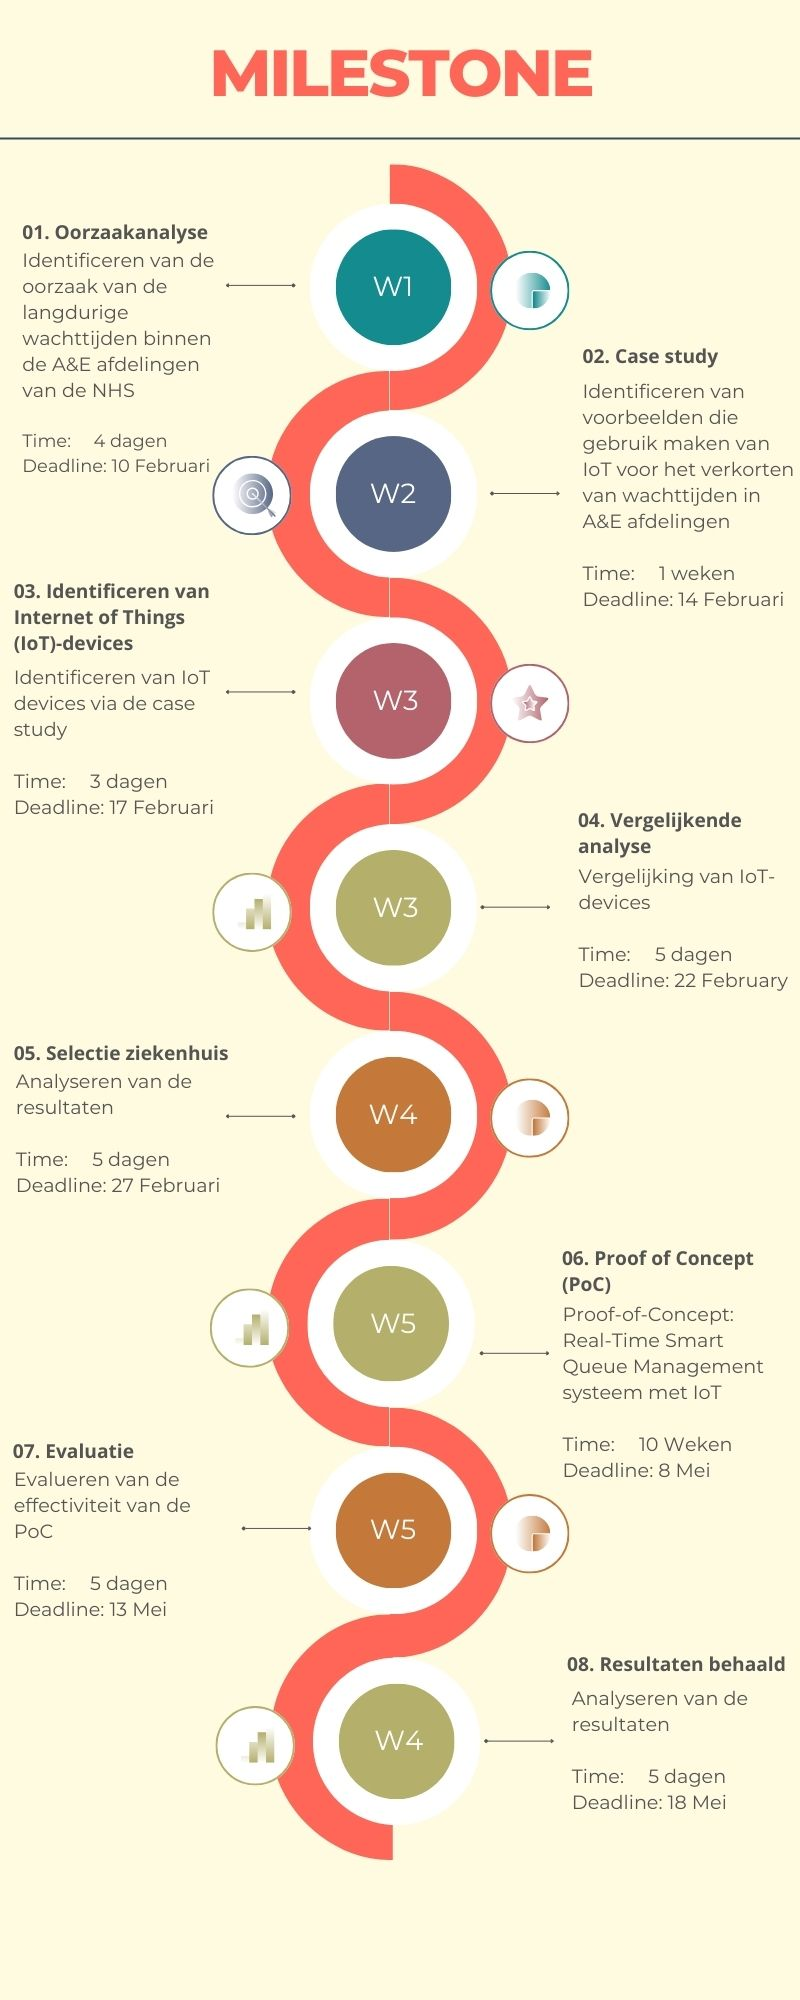
\includegraphics[width=0.92\linewidth]{img/milestone-4.png}
%    \label{fig:Figuur8}
%\end{figure}
